\scanpage{71}
Supposons $\rho$ inv. donc $\unsure{\mathcal E|E}\simeq V\oplus\Delta_0$.

On définit, pour $\lambda$ inv,
\[
\deleted{\unsure{E_{\lambda}}}\quad
p_\lambda:\lambda\overline E\xrightarrow{\sim}V
\]
\diagram{\begin{tikzcd}[ampersand replacement=\&,column sep=large]
x\arrow[r,mapsto]\&\frac1\lambda x-
\tikz[baseline=(c.base)]{\node[draw,ellipse,inner sep=2pt](c){$\dfrac{\Pi}{\rho}$};}
\arrow[d,dash,bend right=30]\\
\&c\quad\text{si }\deleted{\text{\unsure{cela exist}}}
\end{tikzcd}}

Posons
\[
\widetilde s_i=p_1(s_i)=s_i-c\deleted{\unsure{=}}
\]
\[
\left\{\begin{aligned}
\widetilde s_0
&=\deleted{\unsure{-\left[\frac{\sigma}{\rho}a_0+2\right]}}
-\frac1\rho\left[
\deleted{\unsure{a_{-1}}}
\overbrace{\rho'_{n-1,1}}^{\sigma}a_0+
\rho'_{\unsure{n-1|n-2},2}a_1+\mathbin{-}+
\rho'_{n-1,n-1}a_{n-2}+2a_{n-1}+a_n\right]\\
\widetilde s_i
&=\widetilde s_0-\frac1\rho[a_0+\mathbin{-}+a_{i-1}]
\end{aligned}\right.
\]
\margin{$2$ inv}
\[
\widetilde u=p_2(\deleted{\unsure{u}}\inserted{u})
=\frac12u-c=a_{-1}+\frac12a_0-c
=\frac12(\widetilde s_0+\widetilde s_1)
=\widetilde s_0+\frac12a_0
\]
\figure{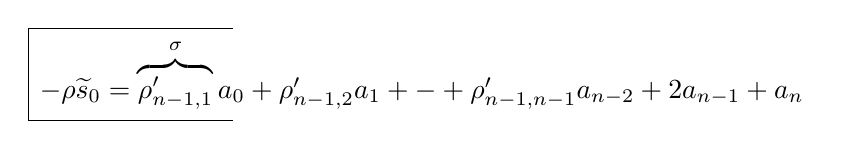
\begin{tikzpicture}
\node[anchor=west,inner sep=4pt](r) at (0,0)
{$-\rho\widetilde s_0=\overbrace{\rho'_{n-1,1}}^\sigma a_0+
\rho'_{n-1,2}a_1+\mathbin{-}+
\rho'_{n-1,n-1}a_{n-2}+2a_{n-1}+a_n$};
\draw ([xshift=2.6cm]r.north west)--(r.north west)--(r.south west)--([xshift=2.6cm]r.south west);
\end{tikzpicture}}
\figure{\begin{tikzpicture}
\node[anchor=west,inner sep=4pt](r) at (0,0)
{$\begin{aligned}
-\rho\widetilde u&=-\rho\widetilde s_0\unsure{-|+}\widetilde\rho a_0
=(\unsure{\sigma|\rho}-\widetilde\rho)a_0+
\rho'_{n-1,2}a_1+\mathbin{-}+
\rho'_{n-1,n-1}a_{n-2}+2a_{n-1}+a_n\\
-2\rho\widetilde u&=(4\widetilde\sigma-\rho)a_0+
2\rho'_{n-1,2}a_1+\mathbin{-}+
2\rho'_{n-1,n-1}a_{n-2}+4a_{n-1}+2a_n
\end{aligned}$};
\draw ([xshift=2cm]r.north west)--(r.north west)--(r.south west)--([xshift=.4cm]r.south west);
\end{tikzpicture}}
\margin{\uline{$n$ pair}\quad$(\rho=2\widetilde\rho)$}
\margin{\unsure{Cas impair}\quad$\sigma=2\widetilde\sigma$}
\[
\widetilde t_i=p_{\unsure{\beta|-\beta}}(t_i)
=-\frac1\beta t_i-c
\]
\[
-\rho\widetilde t_i=+\frac\rho\beta t_i+\Pi
\]
\margin{\unsure{si $i\geqslant1$},
coeff. de $a_0$ est $\deleted{\unsure{4}}-1/\rho$}
\margin{coeff. de $a_n$ est
$-\frac\gamma\beta-\frac1\rho
=-\frac{\beta+\gamma\rho}{\beta\rho}
=-\frac{\sigma\sigma'}{\beta\rho}$}
\[
\begin{aligned}
\text{coeff de }a_{n-1}:\
-\frac{2\gamma-\sigma}{\beta}-\frac2\rho
&=-\frac{2\gamma\rho-\sigma\rho-2\beta}{\beta\rho}\\
&=\frac{-2\sigma\sigma'-\sigma\rho}{\beta\rho}
=-\frac{\sigma}{\beta\rho}[2\sigma'+\rho].
\end{aligned}
\]
\[
-\rho\beta\widetilde t_i=\rho t_i+\beta\Pi\deleted{\unsure{=}}
\]
\[
\begin{aligned}
-\rho\beta\widetilde t_{n+1}
&=\deleted{\rho t_{n+1}+\beta\Pi
=(\rho\gamma+\beta)a_n+
[\rho(2\gamma-\sigma)+2\beta]a_{n-1}+}\\
&\quad\deleted{\unsure{\rho\sigma a_n'{}^*+\rho\gamma\Pi}}\\
&=-\rho\sigma a_n'{}^*
+\underbrace{\rho\gamma\Pi+\beta\Pi}_{\sigma\sigma'\Pi}
\end{aligned}
\]
\margin{$\deleted{2\sigma\sigma'-\rho\sigma=\sigma(2\sigma'-\rho)}$}
\[
\deleted{t_{n+1}=\Theta s_{n+1}'}
=\sigma[\sigma'\underbrace{\Pi}_{a_{n+1}'{}^*}-\rho a_n'{}^*].
\]
\figure{\begin{tikzpicture}
\node[anchor=west,inner sep=4pt](r) at (0,0)
{$-\dfrac{\rho\beta}{\sigma}\widetilde t_{n+1}
=\sigma'a_{n+1}'{}^*-\rho a_n'{}^*=\mathbin{\cdots}$};
\draw (r.north east)--(r.north west)--(r.south west)--(r.south east);
\end{tikzpicture}}
\[
-\frac{\rho\beta}{\sigma}\widetilde t_i
=-\frac{\rho\beta}{\sigma}\widetilde t_{n+1}
+\rho\beta\left(a_n+\beta_{n-1}a_{n-1}+\mathbin{-}
+(\beta_{n-1}\cdots\beta_i)a_i\right)
\]
\mspage{70}

